%!TEX root = main.tex

\chapter{Common Statistical Significance Tests}\label{ch:tests}

The basic idea of common statistical tests in the approach we have taken has been the following:

\be
\i Observe some data
\i Construct a model of the data, with a parameter that needs to be estimated, such as the ``true'' single value ($\mu$, in Section~\ref{sec:estmean}), or the proportion of the event ($\theta$, in Section~\ref{sec:beta}).  
\i Calculate the final, posterior probability of that parameter
\i ``Test'' to see if there is a significant (usually 95\%) probability that the parameter is {\em not} zero\marginnote{In some cases we are not comparing the parameter to \emph{zero} but to some theoretical expectation.  Even there, we are comparing the parameter \emph{minus} the theoretical expectation to zero and thus we don't lose any generality in the procedure by always comparing to zero.}.
\i If the test passes, then one can be reasonably confident that the parameter is non-zero - that the effect is real.  If the test fails, then under the model, the possibility of a zero-effect cannot be reasonably excluded.
\ee

These tests are a subset of the parameter estimation techniques covered in both Chapter~\ref{ch:parameter1} (\emph{\nameref{ch:parameter1}} on page~\pageref{ch:parameter1}) and Chapter~\ref{ch:priors_posteriors} (\emph{\nameref{ch:priors_posteriors}} on page~\pageref{ch:priors_posteriors}), in the special case where we are interested in determining if there is an effect at all.  For example, we might be interested to see if a medical treatment works, so we compare the before- and after-treatment values to see if the difference is non-zero. 

The tests that one typically employs in simple cases go by various names, depending on the model.  This chapter summarizes several of the common ones, and applies them to some typical cases.

\section{$z$-test}\label{sec:ztest}

The $z$-test is the simplest test to use, and is perhaps the most common.  It is used when we have the following assumptions:
\be
\i We are modeling the data as a true value, $\mu$, with uncertainty 
\i We are modeling the as a Normal distribution with \emph{known} deviation, $\sigma$, as in ${\rm Normal}(0,\sigma)$.
\i We are assuming independence between the measurements.
\ee

The model of the data is 
	\beqn
	{\rm data} = \mu + \mbox{uncertainty with probability Normal($\mu=0$,known $\sigma$)}
	\eeqn
where $\mu$ represents the ``true'' value.  The posterior distribution for $\mu$ also follows a Normal distribution, with a smaller uncertainty, $\sigma/\sqrt{N}$ where $N$ is the number of data points.  

To use the $z$-test, we perform the following steps:

\be
\i Calculate our best estimate for $\mu$, denoted as $\hat{\mu}$. 
\i Given the \emph{known} uncertainty, $\sigma$ of a \emph{single} measurement, determine the range of credible values for $\mu$ within the uncertainty of the estimate for the $N$ observations, $\sigma/\sqrt{N}$.  \i Test to see if the credible range includes zero. 
\i If so, then the test passes, and we can be reasonably confident that the parameter is non-zero - that the effect is real. 
\i If the test fails, i.e. the credible range does \emph{not} include zero, then under the model the possibility of a zero-effect cannot be reasonably excluded.
\ee

There are several scenarios where we use the $z$-test, each with the same procedure, differing only in the method of estimating the ``true'' value $\mu$.  

\be
\i  For $N$ independent observations, $x_{1}, x_{2}, \ldots, x_{N}$ we have the best estimate given by the sample mean, and uncertainty related to the single-measurement deviation, $\sigma$, as
\beqn
\hat{\mu} = \frac{x_{1} + x_{2} + \cdots + x_{N}}{N}  \pm \sigma/\sqrt{N}
\eeqn
\i When estimating a proportion, for a large number of events $N$ of which a fraction $f\equiv h/N$ are successful, we have
\beqn
\hat{\mu} &\approx& f \\
\sigma/\sqrt{N} &\approx& \sqrt{f(1-f)/N}
\eeqn
\i For smallish data sets, $5<N<30$, where the uncertainty is \emph{not} known, 
\beqn
\hat{\mu} &\approx&  \frac{x_{1} + x_{2} + \cdots + x_{N}}{N}\\
\sigma/\sqrt{N} &\approx& k S/\sqrt{N}
\eeqn
where we replace the known $\sigma/\sqrt{N}$ from the previous case with an estimate using the sample standard deviation and an adjustment for small data set parameter $k$,
\beqn
S^{2}&=&\frac{1}{N-1}\left( (x_{1}-\bar{x})^{2}+\cdots+(x_{N}-\bar{x})^{2}\right) \\
k&\equiv& 1+\frac{20}{N^{2}}
\eeqn
\ee



\section{What it means and doesn't mean}

For all of these tests, we use the vocabulary of ``statistical significance'', which needs to be further clarified.

\subsection{Significance}

There is a term used in the literature called {\em statistical significance}.\footnote{Although the word ``significant'' occurs in the term ``statistically significant,'' it does not imply that the result itself is important - it may be a small, uninteresting effect, but credibly non-zero.  Perhaps a term like ``statistically detectable'' would be better, but we are unfortunately bound to the historical use of the term.}  Roughly it means a value that is \emph{very unlikely} to be zero (see Table~\ref{table1} on page~\pageref{table1}), or in other words, the value of zero is not within the 95\% percentile.  This is within 2 standard deviations of the value, so the following estimated values are {\em not statistically significant}:
\bi
\i $5\pm 3$ - the \emph{two}-deviation range is [-1,11] contains the value 0
\i $7\pm 4$
\i $-3 \pm 2$
\ei
but the following {\em are statistically significant}:
\bi
\i $5\pm 2$  - the two-deviation range is [1,9] does not contain the value 0
\i $7\pm 3$
\i $-3 \pm 1$
\ei

Statistical significance, at the \emph{very unlikely} level (i.e. 95\% percentile) is often used as a rough guideline to publish a positive effect.  
\begin{table}
\begin{tabular}{cp{1.3in}c}
\parbox{1in}{number of deviations away from zero\\ \ }& term & probability \\\hline\hline
$1\sigma$ & slightly likely/likely & 0.7 (i.e. 7/10) \\
$2\sigma$ & very likely & 0.95 (i.e. 19/20) \\
$3\sigma$ & extremely likely & 0.01 (i.e. 1/100) \\
$>4\sigma$ & virtually certain & $>999,999/1,000,000$
\end{tabular}
\label{tbl:norm likely}
\caption{Rough guide for the conversion of deviations away from zero and the  qualitative labels for probability values for being a \emph{significant} deviation.}
\end{table}


\subsubsection{An unintuitive consequence}

One consequence of this is that two studies that display different magnitudes for a quantity may not be statistically significant in their difference.  The following example is based on an example from Gelman and Hill's book on Data Analysis.\cite{gelman2007data} Say we have two measurements with means and standard deviations:
\bi
\i 25$\pm$10
\i 10$\pm$3
\ei

Further, let us suppose that we are interested in whether the measurements are zero or not.  The first measurement shows a significant effect (the two-deviation range is [5,45] does not contain zero), and the second one does as well (the two-deviation range is [4,16] does not contain zero).  The {\em difference} between them is 
\beqn
(25-10) \pm \sqrt{10^{2}+3^{2}} = 15\pm 10.4
\eeqn
which is {\em not} significant.  One should be careful comparing the magnitudes and uncertainties of measurements!

\section{Student-$t$-test}\label{sec:ttest}

When we are not given the uncertainty of the measurements, $\sigma$, and the data are insufficient to estimate the uncertainty, then we need to estimate both the ``true'' value, $\mu$, and the uncertainty.  This leads to a wider credible range for the ``true'' value.  We can apply the same testing procedure, by looking at the 95\% credible region to see if it includes zero, but this time the posterior distribution we use comes from the so-called Student-$t$ distribution.\marginnote{The odd name ``Student-$t$ test'' comes from the fact the test was originally published by  William Gosset who worked at the Guinness brewery in Dublin and his pen name was ``Student''.}
\be
\i  For $N$ independent observations, we still have the best estimate of the ``true'' value given by the sample mean
\beqn
\hat{\mu} = \frac{x_{1} + x_{2} + \cdots + x_{N}}{N}
\eeqn
\i The best estimate of the uncertainty of a single measurement is given by the sample standard deviation
\beqn
\hat{\sigma} = S 
\eeqn
where $S$ is the sample standard deviation
\beqn
S^{2}&=&\frac{1}{N-1}\left( (x_{1}-\bar{x})^{2}+\cdots+(x_{N}-\bar{x})^{2}\right) 
\eeqn
\i The credible region is determined by the 95\% interval of the posterior, Student-$t$ distribution, of the following form
\beqn
{\rm Student}_{{\rm dof}=N-1}(\bar{x}, S/\sqrt{N})
\eeqn
\i Test to see if the credible range includes zero. 
\i If so, then the test passes, and we can be reasonably confident that the parameter is non-zero - that the effect is real. 
\i If the test fails, i.e. the credible range does \emph{not} include zero, then under the model the possibility of a zero-effect cannot be reasonably excluded.
\ee



\section{Computer Examples}
\begin{fullwidth}
\begin{lstlisting}
from sie import *
\end{lstlisting}

\begin{lstlisting}
data=load_data('data/iris.csv')
\end{lstlisting}

\begin{lstlisting}
x_sertosa=data[data['class']=='Iris-setosa']['petal length [cm]']
\end{lstlisting}

\begin{lstlisting}
x=x_sertosa
mu=sample_mean(x)
N=len(x)
sigma=sample_deviation(x)/sqrt(N)
t_sertosa=tdist(N,mu,sigma)

print "total number of data points:",N
print "best estimate:",mu
print "uncertainty:",sigma
\end{lstlisting}

\begin{verbatim}
total number of data points: 50
best estimate: 1.464
uncertainty: 0.0245381834898
\end{verbatim}

\begin{lstlisting}
new_length=1.7
\end{lstlisting}

\begin{lstlisting}
distplot(t_sertosa,label='petal length',xlim=[1.37,1.8],
                 quartiles=[.01,0.05,.5,.95,.99],
)
ax=gca()
ax.axvline(1.7,color='r')
savefig('../../figs/z_test_iris.pdf')
\end{lstlisting}

\begin{verbatim}
<matplotlib.figure.Figure at 0x10f9d2710>\end{verbatim}

\begin{center}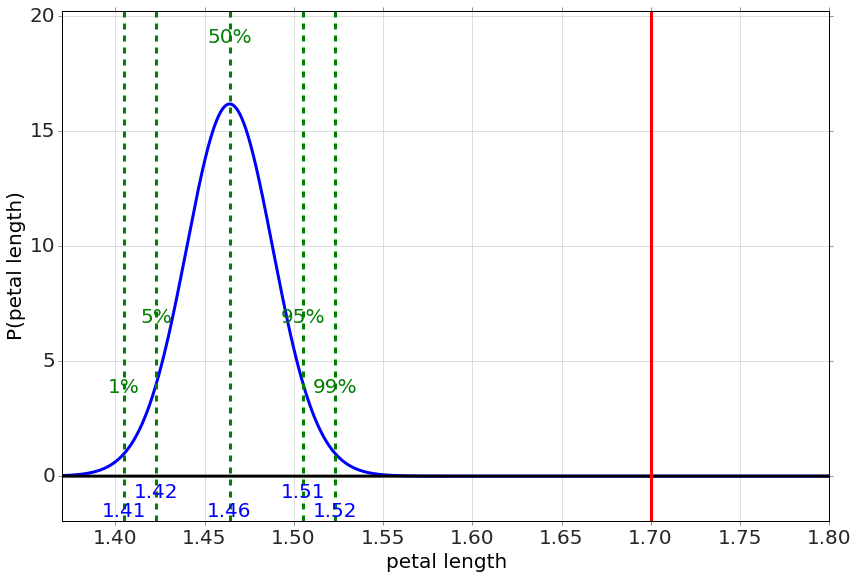
\includegraphics[width=4.5in]{Common_Significance_Tests/Common_Significance_Tests_fig0.png}\end{center}

\begin{lstlisting}

\end{lstlisting}


\end{fullwidth}